\section{Results}

Our Tweether system succinctly shows regional weather characteristics and local sentiment classification using a layered design. The edge bundling method can create smooth curves with coherent shapes and avoid visual clutter. The resulting visualization is visually aesthetic as well as directs a user's focus of attention to salient relationship between weather and mood over geographic locations and time. We implemented Tweether using JavaScript and WebGL such that the system can be viewed from any devices supporting HTML5 and WebGL. 

%We have two goals in our case studies. First, we want to determine if there is any correlation between weather and mood. Second, we would like to verify if our predicted mood is correct.

%\begin{figure*}[htp]
%  \centering
%  \subfigure[Temperatures in Omaha and Lincoln]{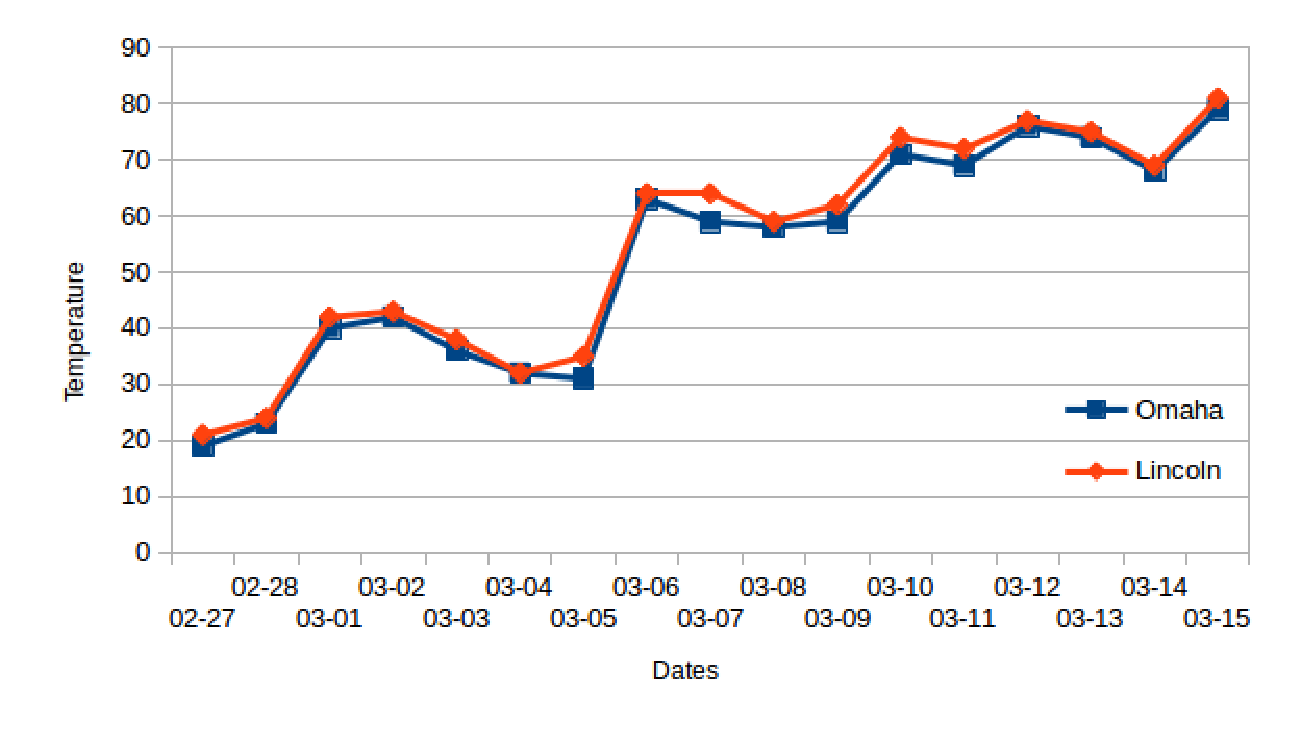
\includegraphics[scale=0.25]{chart1}}\quad
%  \subfigure[Sentiment of Omaha and Lincoln Tweets]{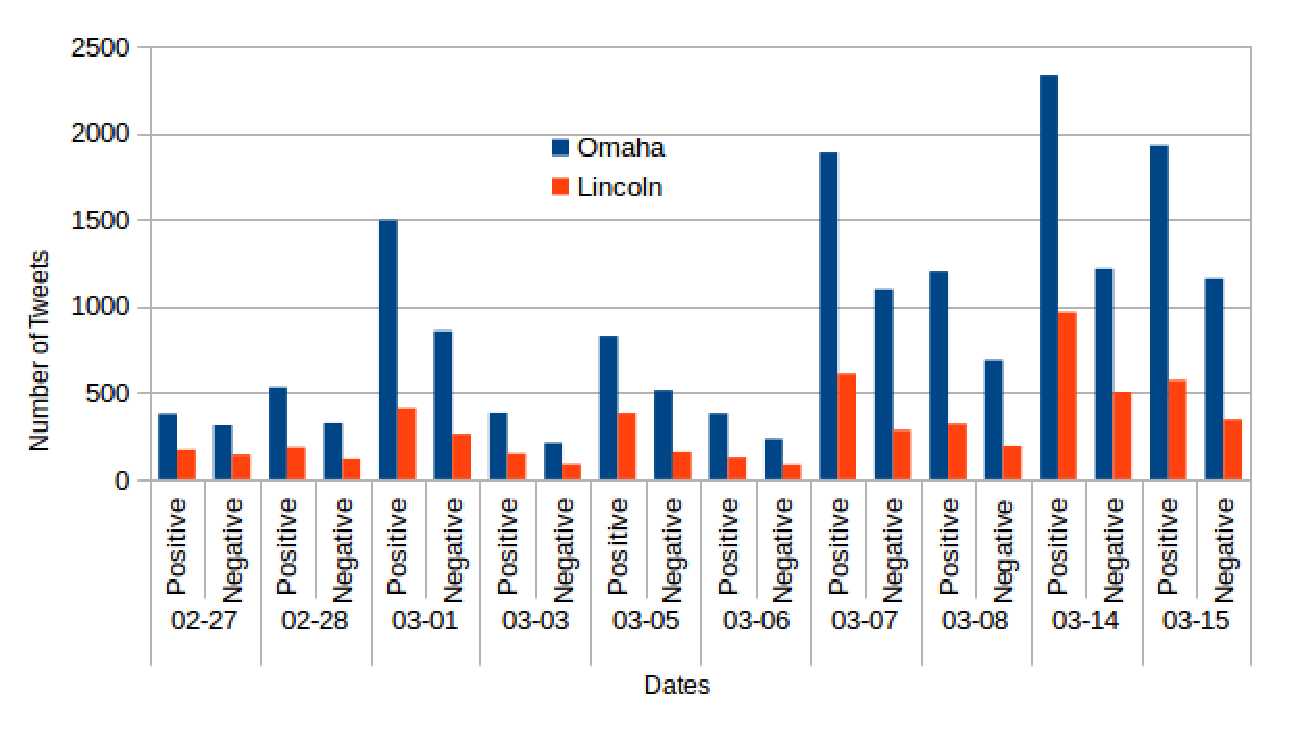
\includegraphics[scale=0.25]{chart2}}\quad
%  \subfigure[Sentiment of Omaha and Lincoln Tweets]{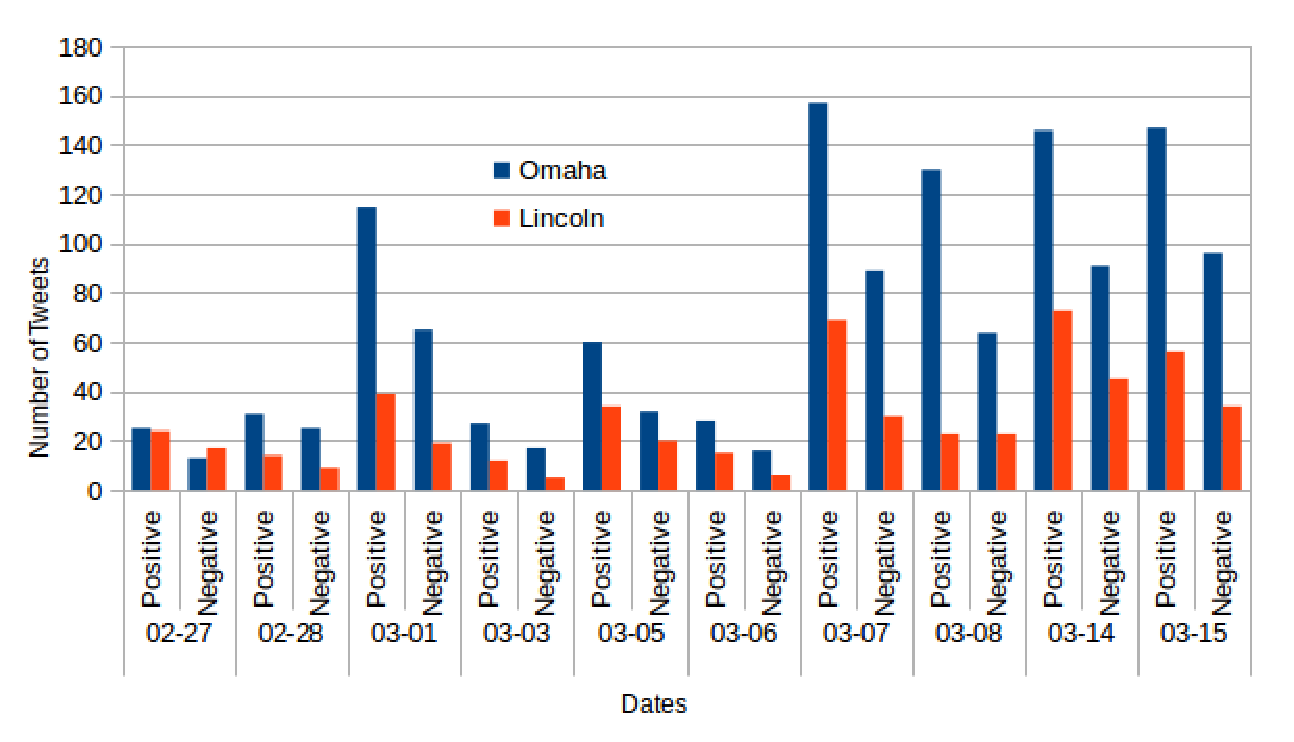
\includegraphics[scale=0.25]{chart3}}
%\caption{The comparison of weather to sentiment.}
%\label{fig:chart_1}
%\end{figure*}
%


\subsection{Tweet Weather Correlation}

%We use two data sets to show our visualization.
We use the weather and twitter data from two back to back weekends (from March 6th to March 8th, and from March 13rd to March 15th) to see if there is any relationship between the temperature and the overall mood of people. We are lucky that the days we chose show warmer changes with certain fluctuations in weather. Being on the brink of Spring, we predict that the overall Tweets for the warmer weekend will have a more positive sentiment in comparison to the colder weekend. This weather pattern also can show any potential correlation for seasonal affective disorder (SAD)~\cite{denissen2008effects}.

\subsubsection{All Tweets}

In the first study, we use all collected tweets whether a tweet contains weather-related terms or not. Figure~\ref{fig:teaser}


%------------------------------------------------
\begin{figure}[t]
\begin{center}
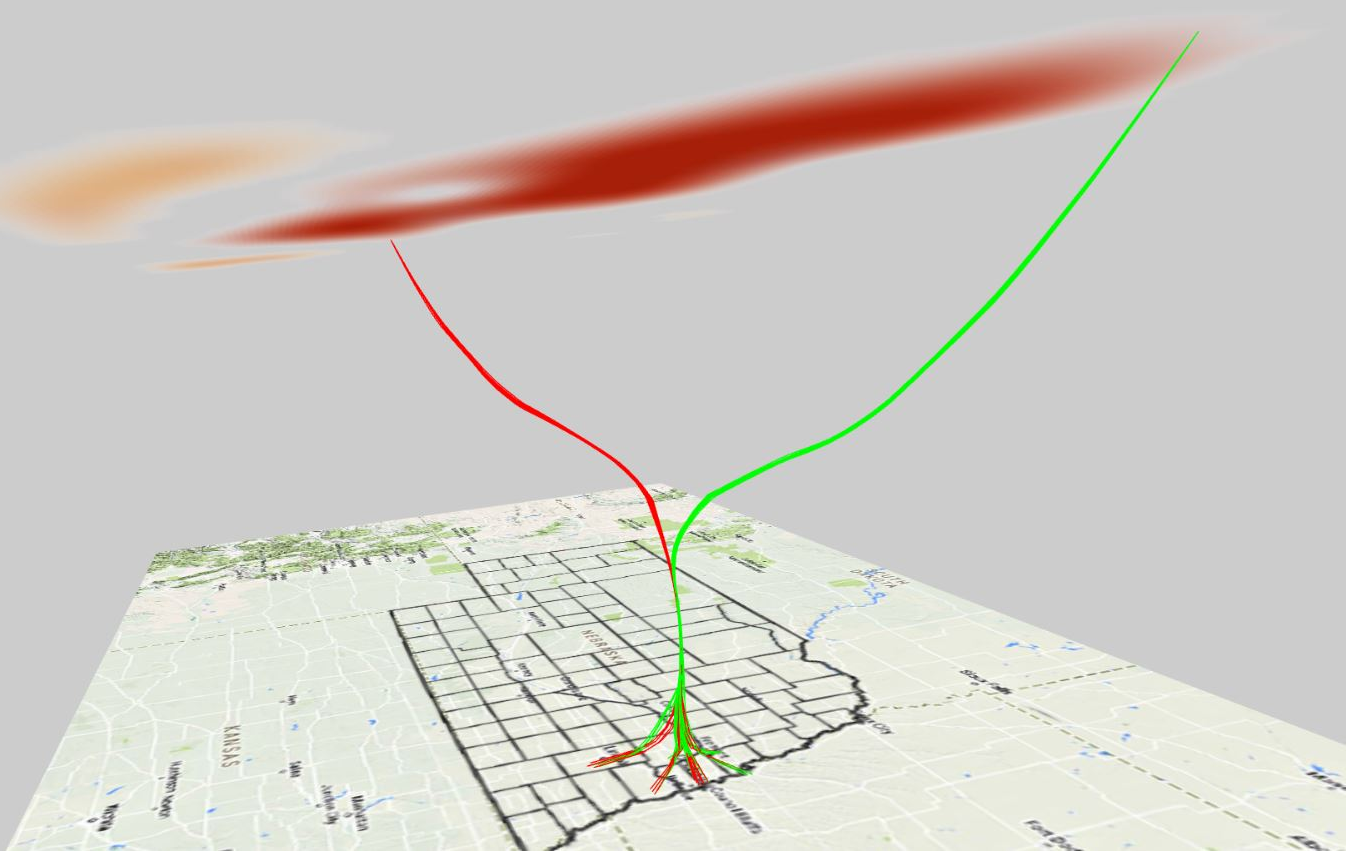
\includegraphics[width=1.0\linewidth]{wk1-real_cr.png} \\
\mbox{\small{(a)}}\\
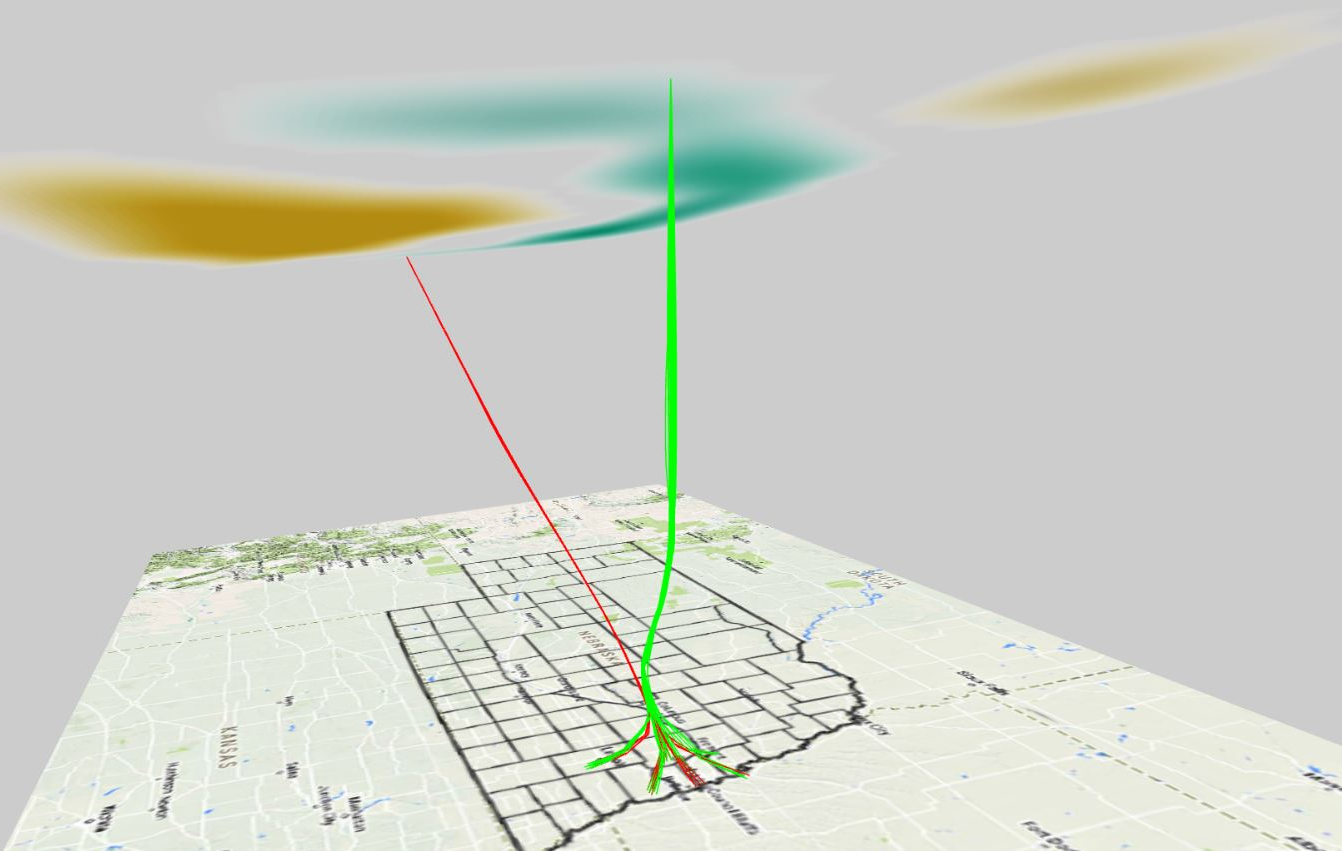
\includegraphics[width=1.0\linewidth]{wk2-real_cr.png} \\
\mbox{\small{(b)}}
\end{center}
\vspace{-.1in}
\caption{The visualization results at two time steps, (a) 1pm on March 8th and (b)1pm on March 15th.}
\label{fig:cities}
\end{figure}
%------------------------------------------------

Of all the cities, we see that Omaha and Lincoln have the most tweets, and thus we use these two cities to show the details of our results. We choose to look at times where most of the population is awake (i.e., noon to 11 PM). Figure~\ref{fig:cities} shows the visualization results at two time steps over the two week ends. The color values from indigo to dark orange are computed according to the local TSK values. From Figure~\ref{fig:cities} (a), we can see that the tweets have a equal amount of positive and negative sentiments, and they are all mapped to the same primary weather cluster that has the highest local TSK. We note this cluster is the dominant weather pattern nearly covering the entire state of Nebraska. From Figure~\ref{fig:cities} (b), we can see that the majority of tweets have the positive sentiment within these two cities. They are all mapped to the same primary weather cluster that has the lowest local TSK. In addition, from both the images, we can see that the most red lines (negative sentiment) came from Omaha. By visualizing multiple time steps, we observe that both the temperature and the total number of tweets become higher with an increase of positive sentiment and a decrease of negative sentiment.

%------------------------------------------------
\begin{figure}[t]
\begin{center}
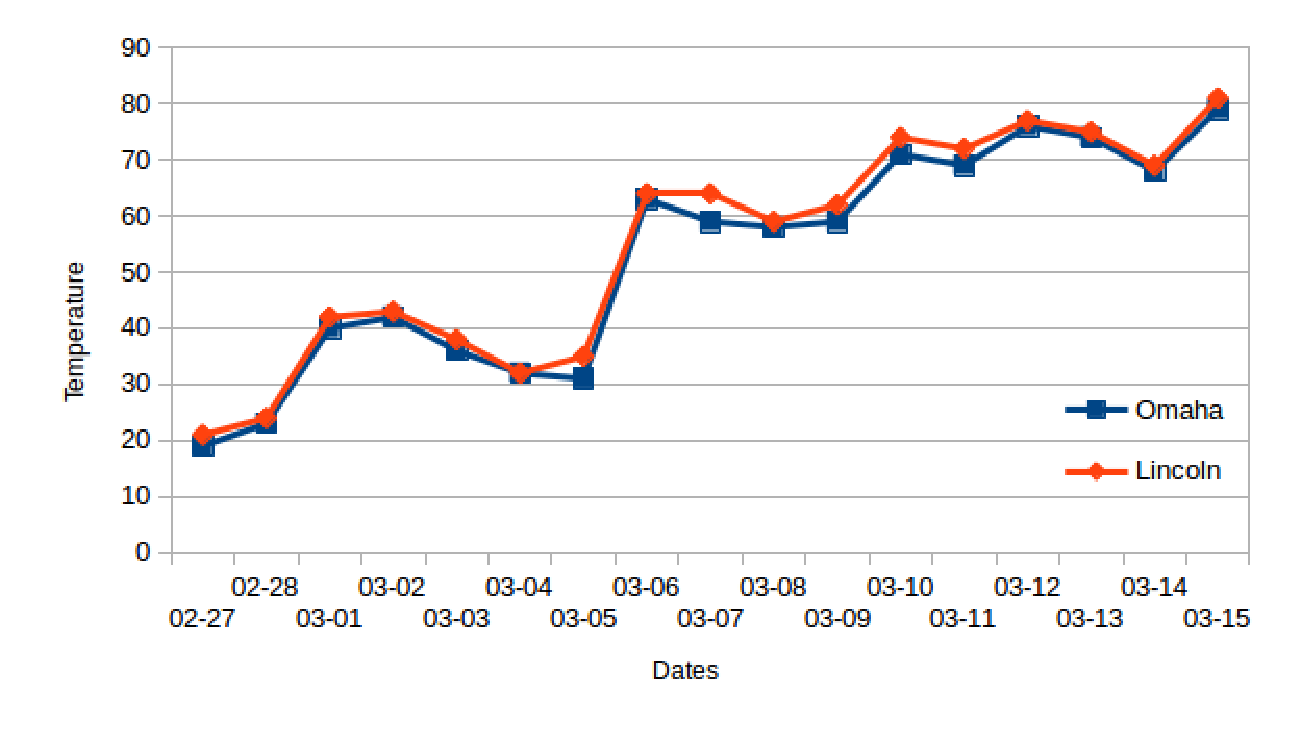
\includegraphics[width=1.0\linewidth]{chart1} \\
\mbox{\small{(a)}}\\
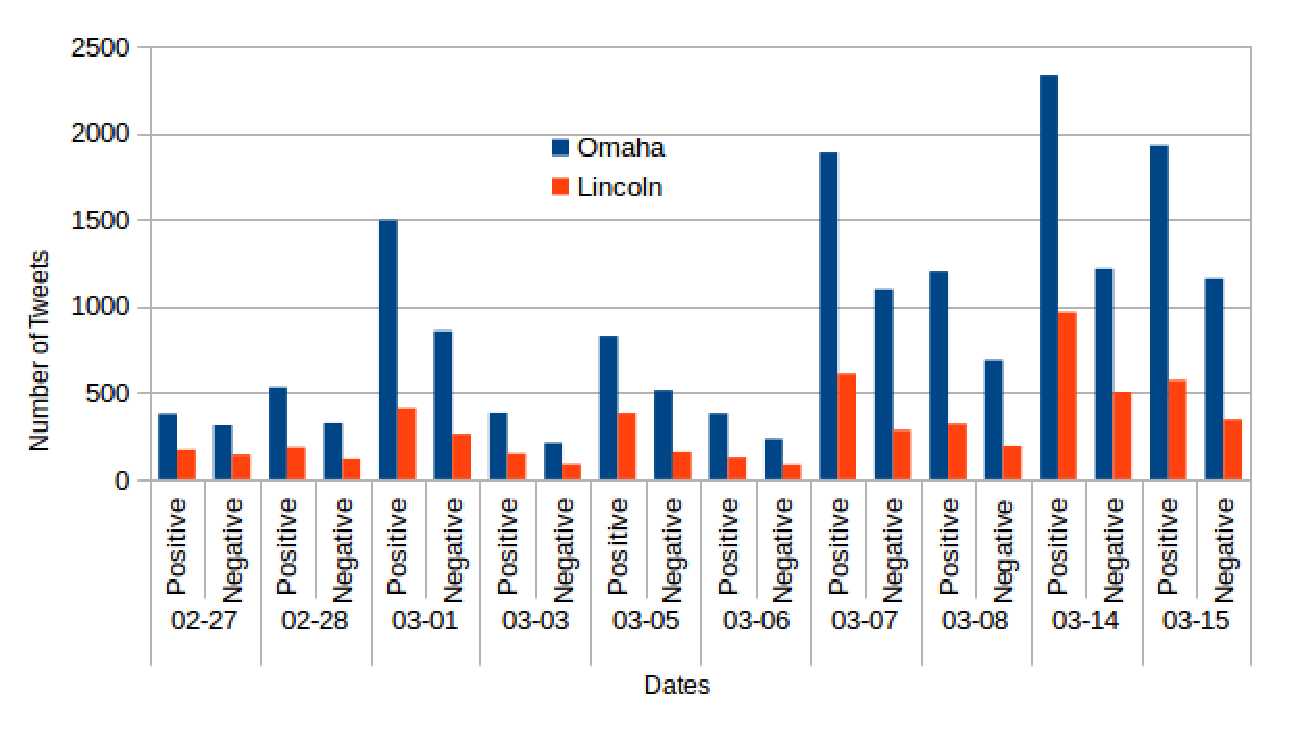
\includegraphics[width=1.0\linewidth]{chart2} \\
\mbox{\small{(b)}}\\
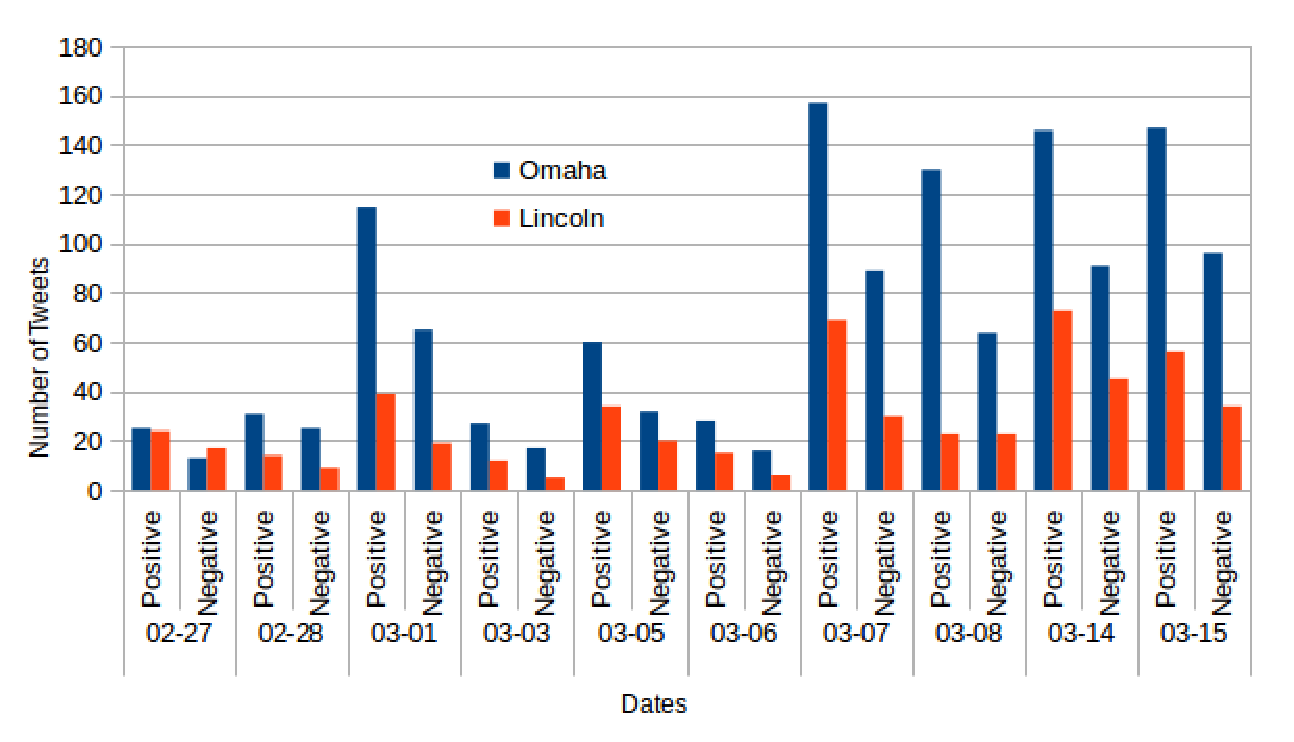
\includegraphics[width=1.0\linewidth]{chart3} \\
\mbox{\small{(c)}}
\end{center}
\vspace{-.1in}
\caption{The comparison of weather to sentiment.}
\label{fig:chart_1}
\end{figure}
%------------------------------------------------

To explain our observation, we examine the detailed weather patterns, as shown in Figure~\ref{fig:chart_1} (a). Overall it shows a dramatically growing trend of temperature, roughly from $20^\circ$F to $80^\circ$F, as well as some fluctuations around the early March. From Figure~\ref{fig:chart_1} (b) we can see the tweets and their sentiment for select days through the two weeks, where more emphasis is placed on the first week and less on the later. Each date has a positive and negative count, where we clearly see a throughout pattern that the positive tweets outweigh the negative tweets. Another pattern that we see is that as the temperature increases the number of tweets increase. We also observe that more people tweet on Saturday than on Sunday. We think that this may be related to a number of factors: people go to church on Sunday where they choose to be among family, they do work around the house, or they do not have any eventful things which they feel they need to share.

We do not see that with the change of temperature that there is a clear trend of more positive tweets versus negative tweets. The number of positive tweets is at least more than half the amount of negative tweets. We observe that the percentage of the negative sentiment is higher in the colder temperatures than in the warmer temperature. For example, the weekend of March 14h has the highest temperatures as shown in Figure~\ref{fig:chart_1}(a), and the percentage of negative sentiment is lowest as shown in Figure~\ref{fig:chart_1}(b). However, from the statistics in Figure~\ref{fig:chart_1} (b), we cannot be certain if there is a clear correlation. To address this issue, we look at tweets only with words related to weather to see if we find any trends.

\subsubsection{Weather Related Tweets}

Other than using all the tweets we collected, we filter them for weather-related terms (i.e., snow, sunny, warm, cold, rain, etc.). We want to see if there is a stronger correlation in this situation compared to using all the tweets. %In this situation, we are unfortunately limited to a few tweets. 
As shown in Figure \ref{fig:chart_1}(c), we see that the number of tweets drastically reduces to around 160 tweets for one day.
%Fortunately, we are able to see a pattern with weather and positive tweets. 
We note that there is also a spike of tweets when there is warmer weather (e.g., the weekend of March 14th). This pattern is seen in both sets of tweet data sets. However, we are now able to confirm that the correlation is due to weather. As the weather increased slightly on March 1st we see a spike in amount of tweets overall (Figure \ref{fig:chart_1}(b)) and also when the tweets had weather-related words (Figure \ref{fig:chart_1}(c)). We can also see that in Figure \ref{fig:chart_1}(c) that with the warmer weather the number of tweets in relation to the weather increases by approximately twice the amount. We still see the trend of more positive tweets in comparison to negative tweets when using the filtered data set.

However, this trend can be clearly conveyed in our visualization (Figure~\ref{fig:cities}) without an examination of detailed statistics which can be cumbersome for large tweet data.


\subsection{Prediction}
\label{sec:caseprediction}

Using the same data set we select a subset of two weekends to determine if the predicted value is close to the outcome. We choose March 6th, 7th and 8th for weekend one and March 13th, 14th and 15th for weekend two. The first weekend has between 10 to 20 degrees difference to the second weekend to take into account any change in weather patterns. We collect our predictions for Saturday and Sunday and compare them to the real sentiment of each hour. Again we focus on the two most populous cities in Nebraska, Lincoln and Omaha.

Figure~\ref{fig:predict} shows the results of the three methods described in Section~\ref{sec:pred} at two time steps. The ground truth is shown in Figure~\ref{fig:cities}. Figure~\ref{fig:predict} (a) and (b) are generated using the first method where we only consider the temperature difference. As we use the same locations, intuitively the images are close to the ground truth. Figure~\ref{fig:predict} (c) and (d) are generated using the second method where we only consider the time difference, while Figure~\ref{fig:predict} (c) and (d) are based on the third method with considering both the temperature and time differences. We note that the thickeners of line bundles are most similar to the ground truth. 

Table~\ref{tab:err} provides a quantitative measure of errors for the three methods. We compare the number of predicted positive (negative) tweets at each time step to the ground truth. The percentage number is the relative error. We can see that the third method has the least errors for both positive and negative tweets. The second method has the worst error percentage. This is primarily due to the fact that we do not take into account the weather. Because it uses the temperature, the first method has the slight better performance than the second method.

%------------------------------------------------
\begin{figure}[t]
\begin{center}
$\begin{array}{c@{\hspace{0.01\linewidth}}c}
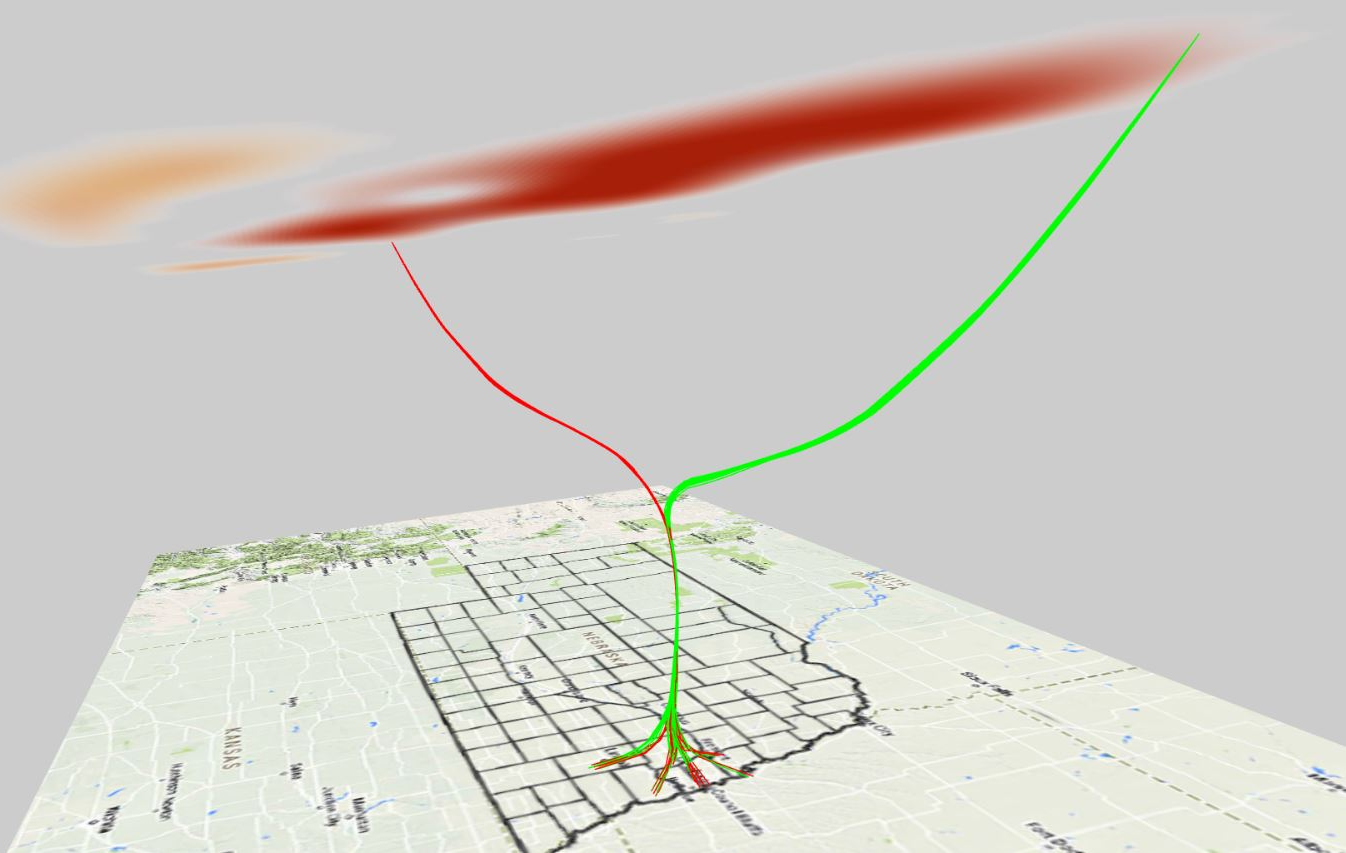
\includegraphics[width=0.49\linewidth]{wk1-m1_cr.png} &
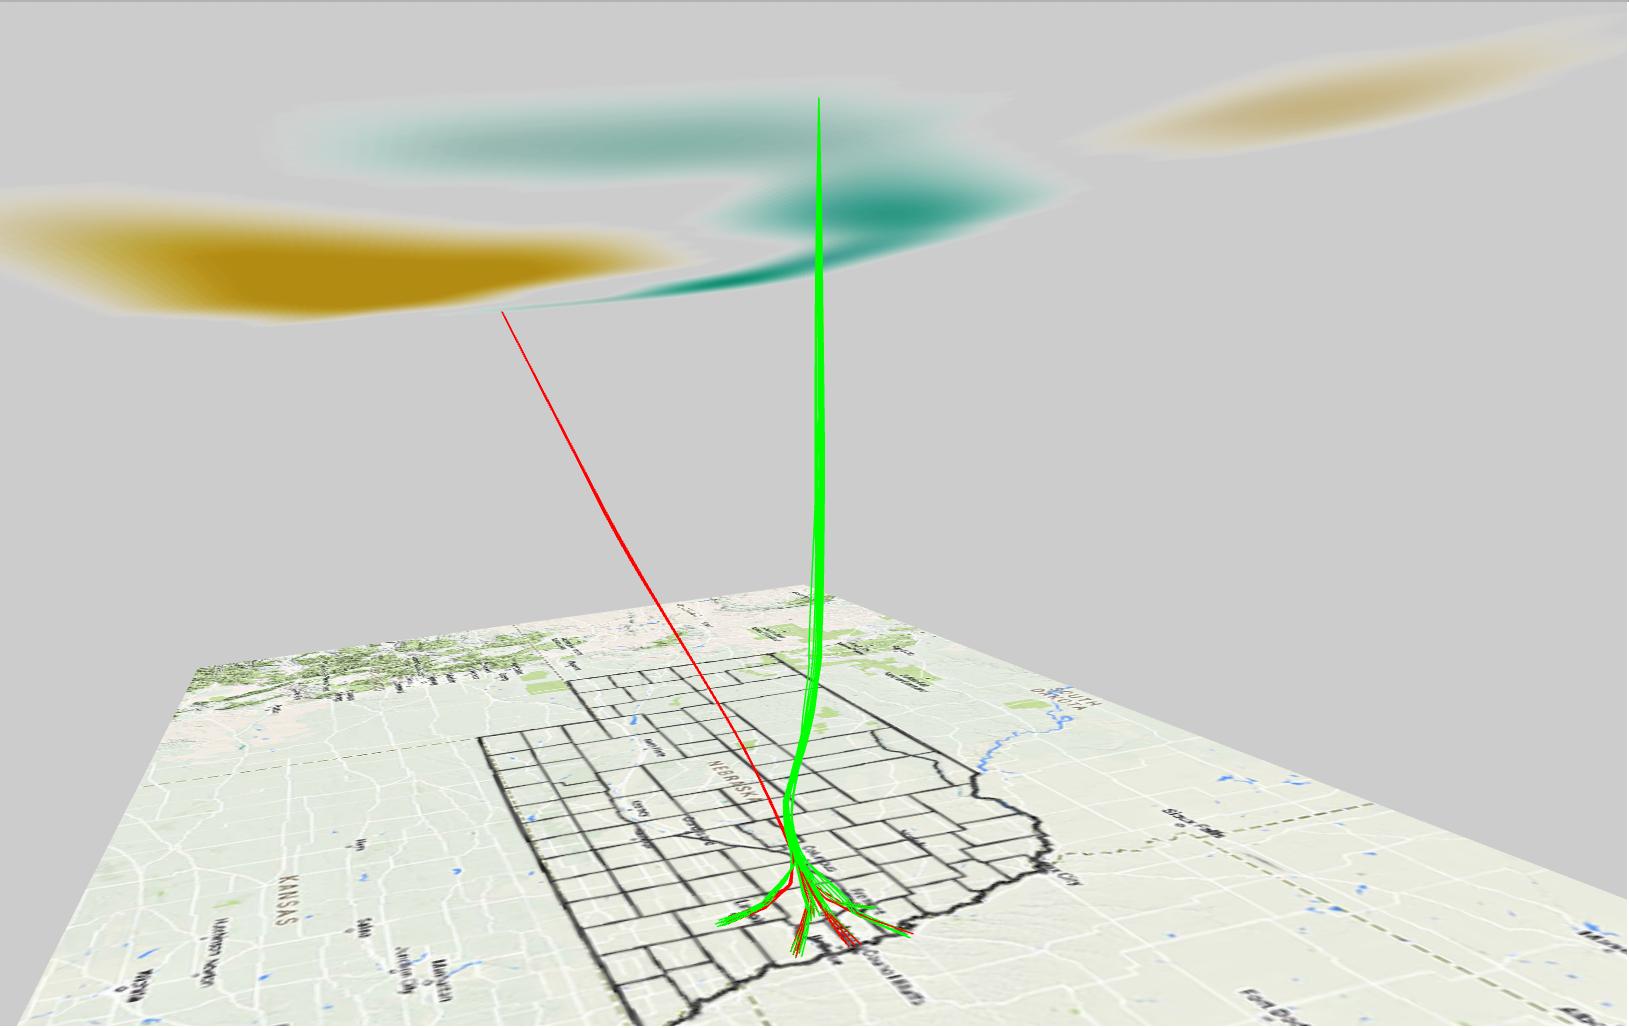
\includegraphics[width=0.49\linewidth]{wk2-m1_cr.png}
\\
\mbox{\small{(a)}} & \mbox{\small{(b)}}
\\
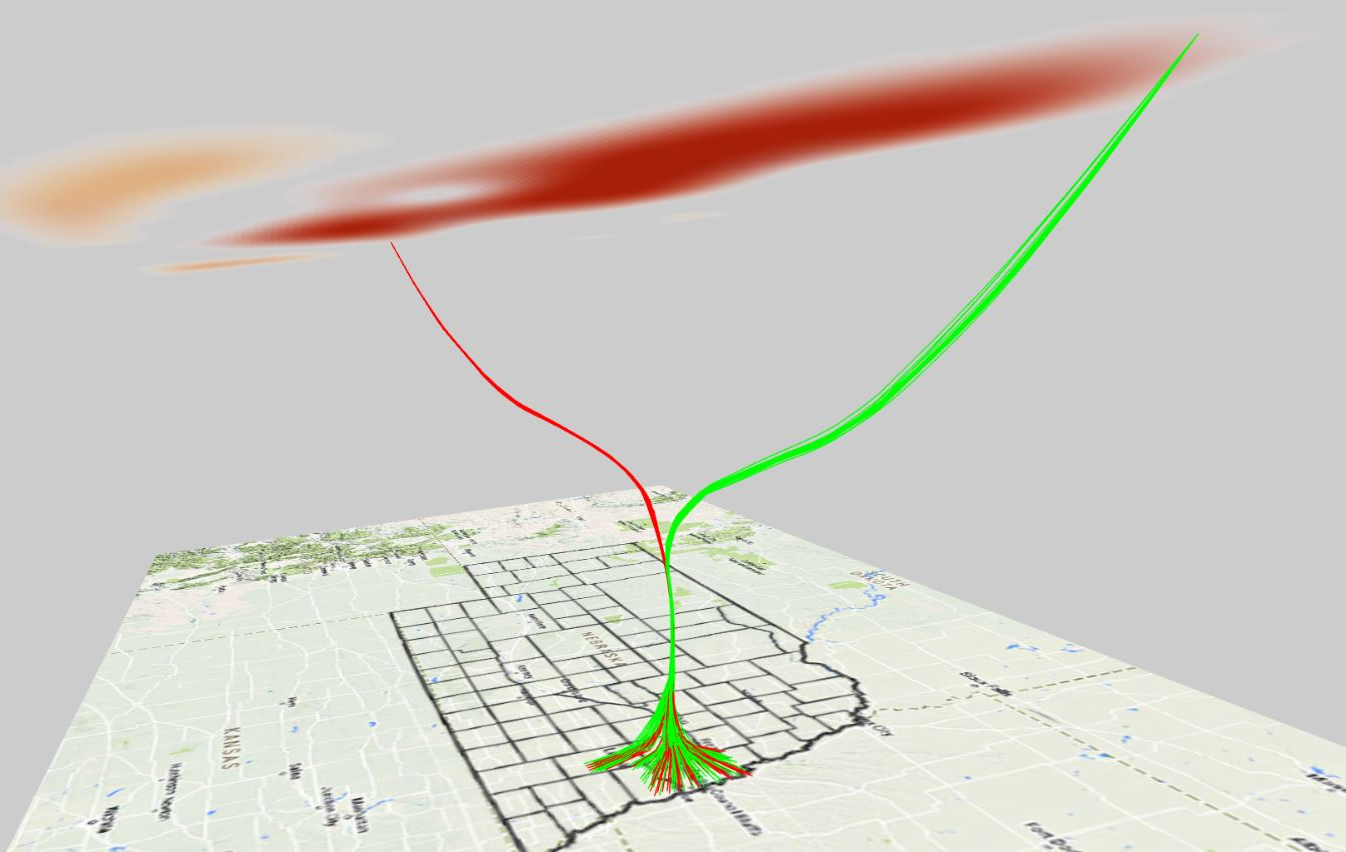
\includegraphics[width=0.49\linewidth]{wk1-m2_cr.png} &
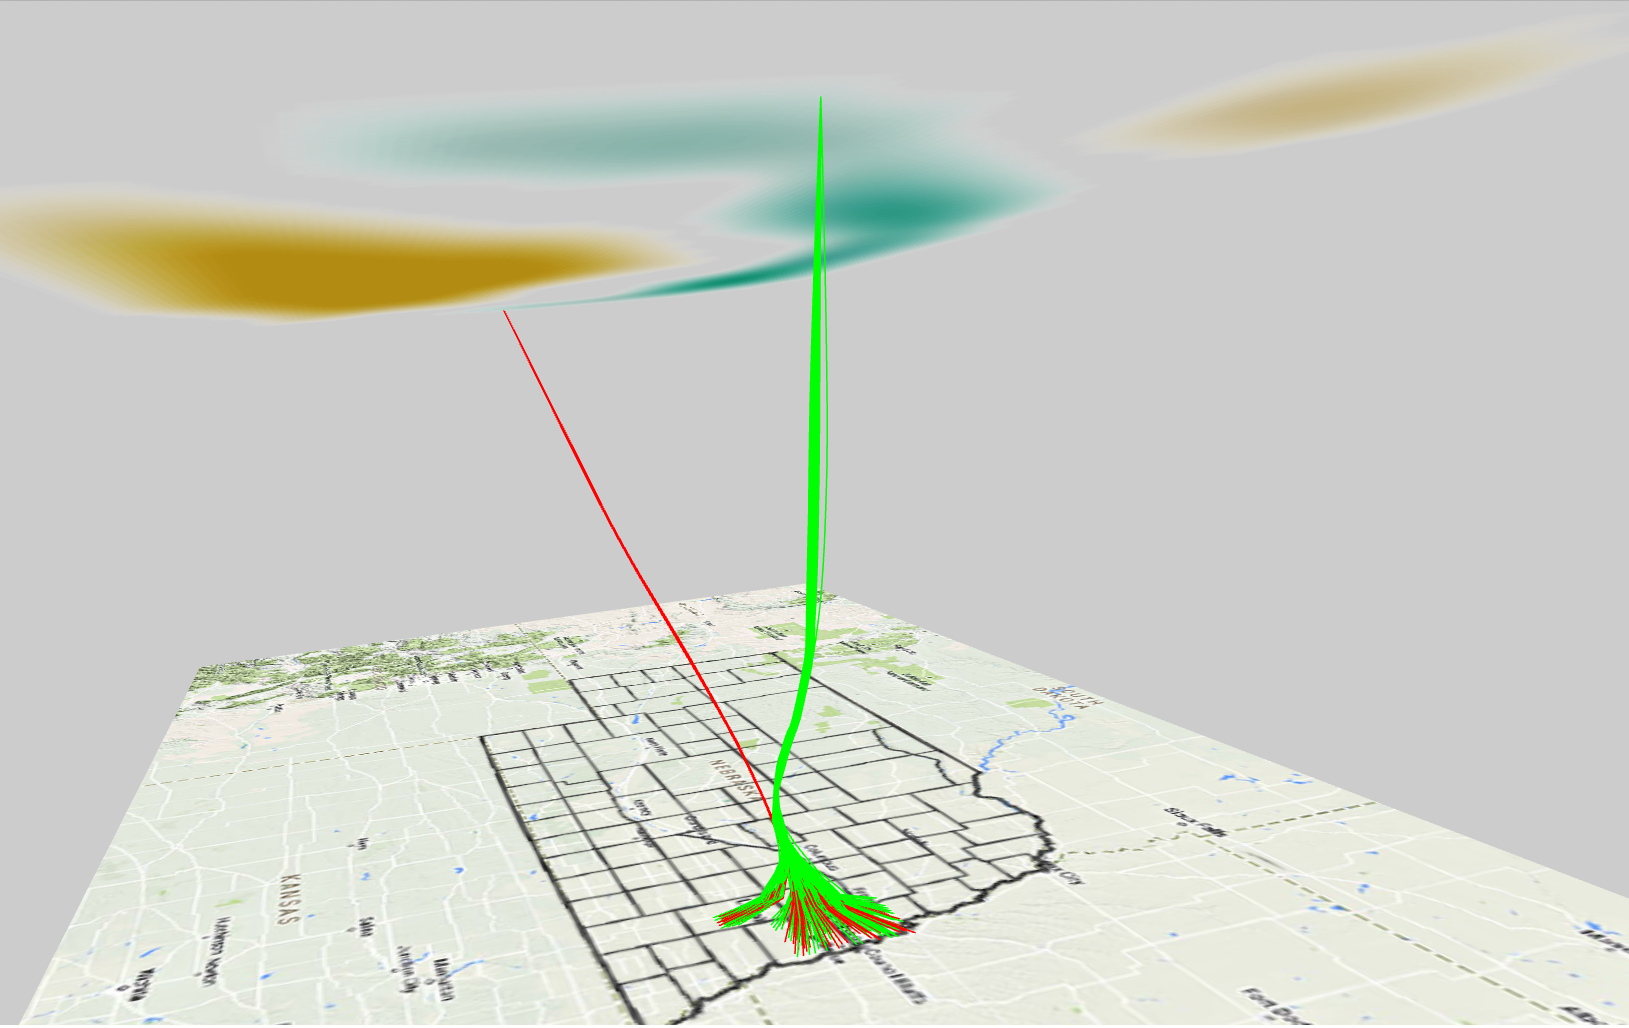
\includegraphics[width=0.49\linewidth]{wk2-m2_cr.png}
\\
\mbox{\small{(c)}} & \mbox{\small{(d)}}
\\
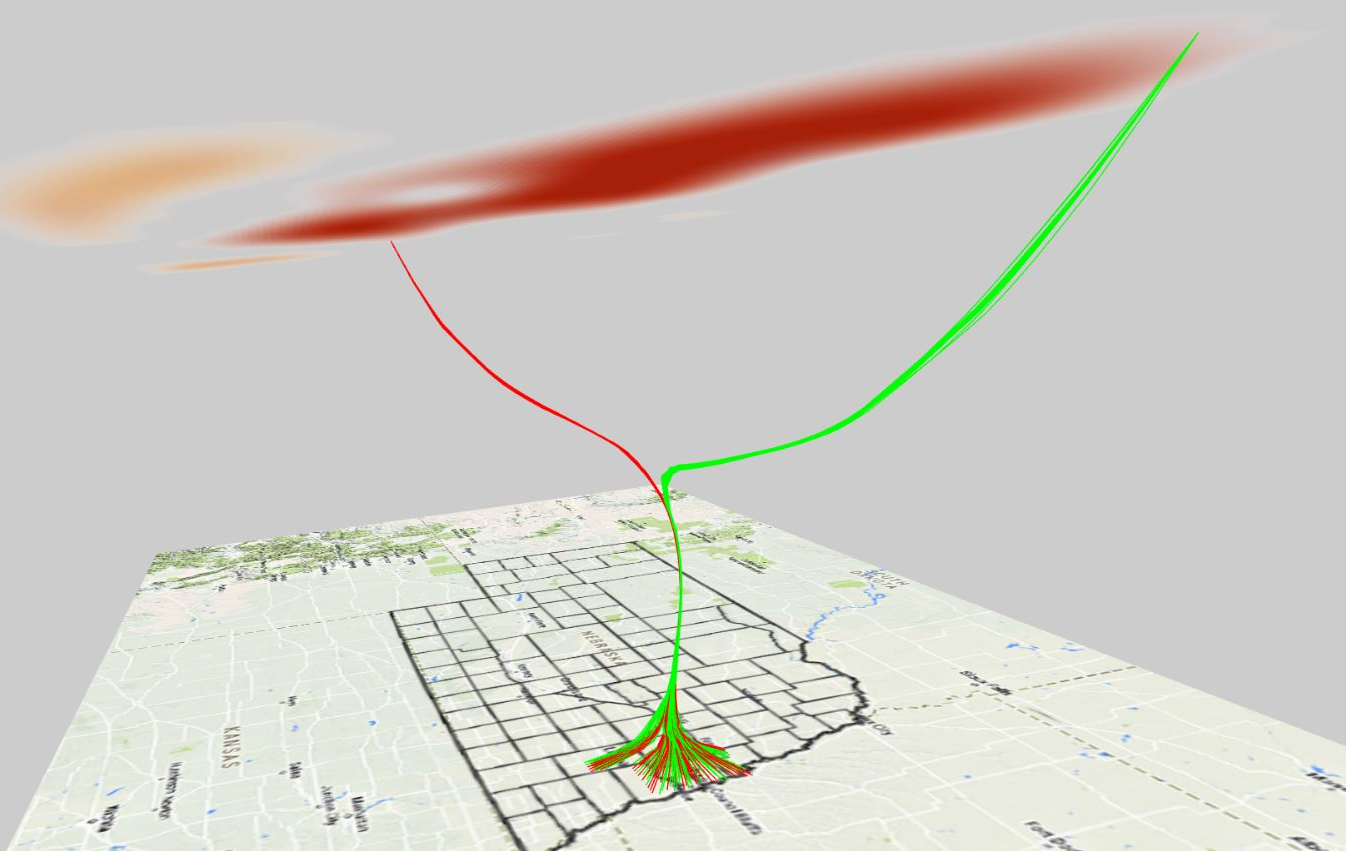
\includegraphics[width=0.49\linewidth]{wk1-m3_cr.png} &
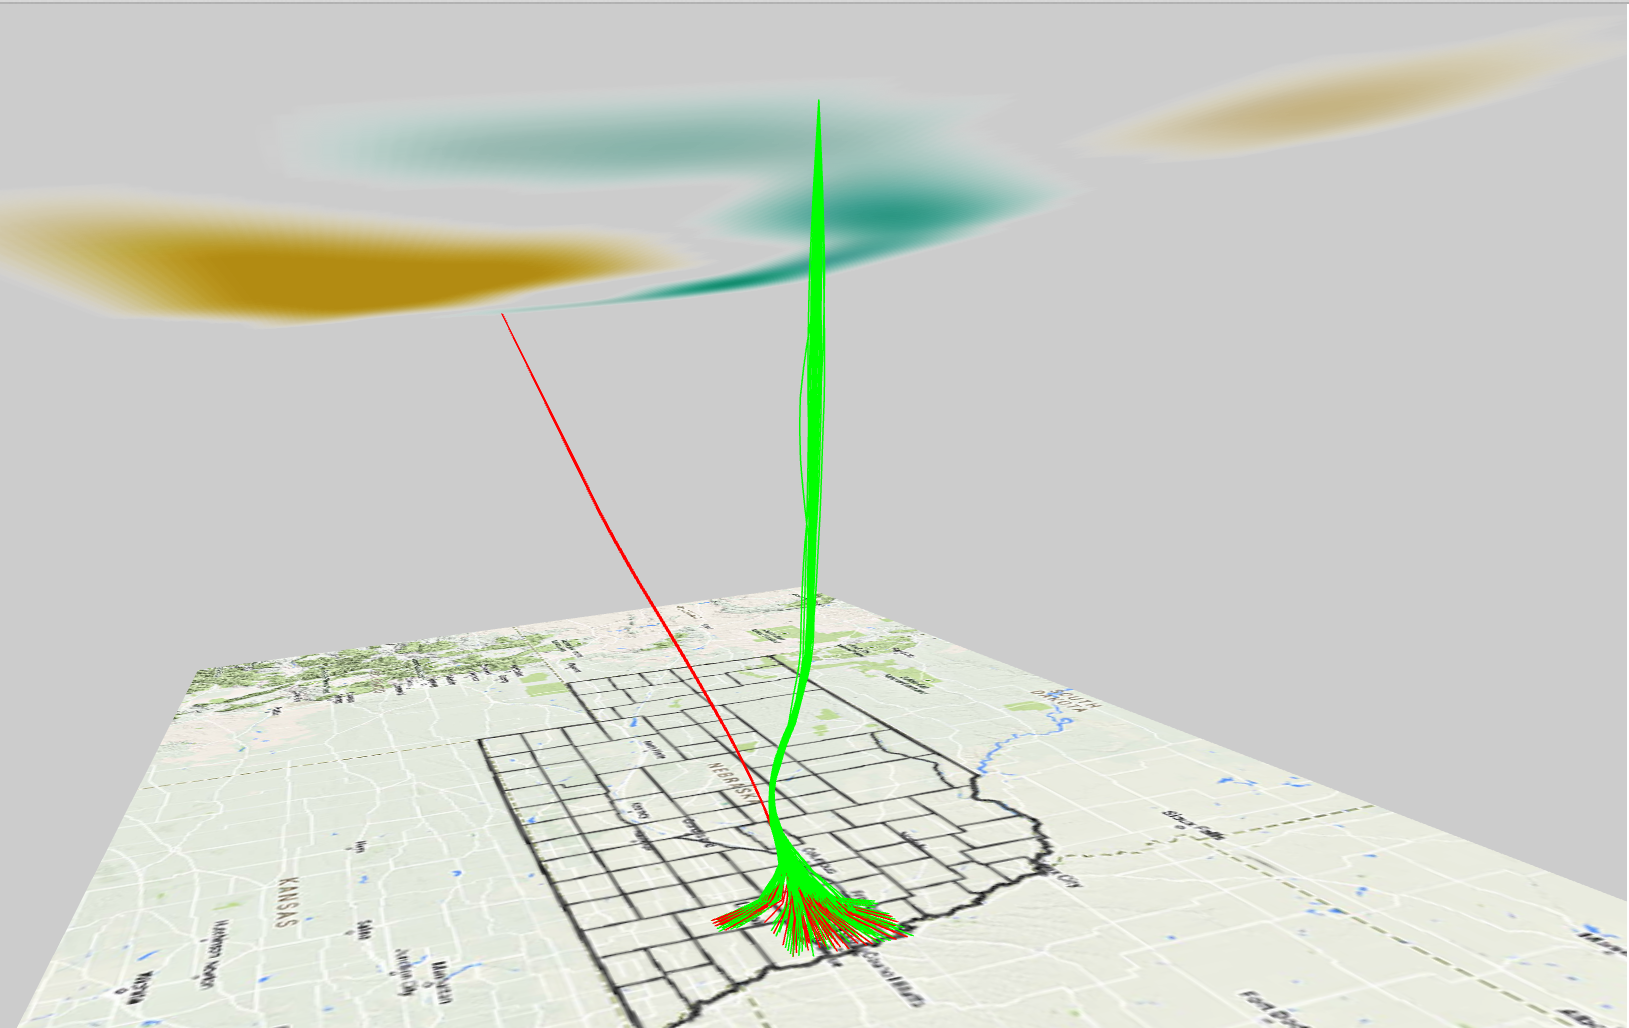
\includegraphics[width=0.49\linewidth]{wk2-m3_cr.png}
\\
\mbox{\small{(e)}} & \mbox{\small{(f)}}
\end{array}$
\end{center}
\vspace{-.1in}
\caption{The results of three prediction methods. (a), (c), and (e) correspond to the predicted results of 1pm on March 8th. (b), (d), and (f) correspond to the predicted results of 1pm on March 15th.}
\label{fig:predict}
\end{figure}
%------------------------------------------------

%----------------------------------
\begin{table}[t]
\caption{The percentage errors of three prediction methods.}
%\vspace{-.1in}
\begin{center}
\scalebox{1}{
\addtolength{\tabcolsep}{-4pt}
\begin{tabular}{|l||r|r|}
\hline
 & Positive & Negative  \\ \hline
Method 1 & 23\% & 27\% \\ \hline
Method 1 & 26\% & 28\% \\ \hline
Method 1 & 23\% & 26\% \\ \hline
\end{tabular}}
\end{center}
\vspace{-.2in}
\label{tab:err}
\end{table}
%----------------------------------



